\chapter{Hasil dan Pembahasan}

Bab ini menjelaskan hasil dan pembahasan penelitian yang digunakan untuk melakukan evaluasi komparatif terhadap berbagai strategi \textit{retrieval} dan teknik \textit{reranking} dalam sistem \textit{information retrieval}. Penelitian ini berfokus pada analisis kinerja pendekatan \textit{hybrid retrieval} yang menggabungkan metode \textit{dense} dan \textit{sparse}, penerapan \textit{cross-encoder} sebagai mekanisme \textit{reranking}, serta eksplorasi kombinasi keduanya melalui skema pembobotan (\textit{alpha}) untuk mengoptimalkan relevansi hasil pencarian. Pembahasan dalam bab ini mencakup penjelasan mengenai perancangan basis pengetahuan berbasis dokumen ISO/IEC 27001:2022, proses penyusunan \textit{dataset} variasi \textit{query} untuk kebutuhan evaluasi, perancangan metode \textit{hybrid retrieval} beserta pengembangannya menggunakan pendekatan \textit{cross-encoder reranking}, serta analisis hasil pengujian berdasarkan variasi parameter dan variabel independen yang digunakan pada penelitian.

\section{Inisiasi dan Konfigurasi Lingkungan Penelitian}

\subsection{Pembangunan Basis Pengetahuan ISO 27001}

Basis pengetahuan pada penelitian ini dibangun dengan mengumpulkan dan menyusun informasi terkait kontrol keamanan dari standar ISO/IEC 27001:2022, khususnya pada Annex A domain A.5 (\textit{Organizational Controls}), A.6 (\textit{People Controls}), A.7 (\textit{Physical Controls}), dan A.8 (\textit{Technological Controls}). Seluruh dokumen yang digunakan sebagai sumber pengetahuan (\textit{corpus}) disimpan dalam format JSON (\textit{JavaScript Object Notation}), di mana setiap kontrol direpresentasikan sebagai satu entitas data yang terdiri dari atribut deskriptif, indikator audit, serta kata kunci dalam dua bahasa (Bahasa Inggris dan Bahasa Indonesia). Struktur data JSON yang digunakan telah dijelaskan pada Tabel~\ref{tab:json_struktur} di Subbab 3.2.1.

\subsection{Pembangunan \textit{Ground Truth} dan Variasi \textit{Query}}

\textit{Query} dan \textit{ground truth} disusun sebagai komponen utama dalam proses evaluasi \textit{retrieval} sistem. Penyusunan kumpulan \textit{query} dilakukan dalam dua kategori, yaitu \textit{query} sintetis dan \textit{query} asli berdasarkan dokumen DTI UGM. Variasi \textit{query} sintetis dirancang berdasarkan kombinasi dua variabel, yaitu variasi panjang (pendek dan panjang) serta variasi level eksplisitasi (eksplisit dan implisit), sehingga menghasilkan empat jenis variasi \textit{query} yang telah dijelaskan pada Tabel~\ref{tab:jenis_query} di Subbab 3.2.2.

Total \textit{dataset} yang digunakan berjumlah 250 \textit{query} sintetis, dengan distribusi \textit{ground truth} yang merata antar \textit{annex control} pada domain A.5 hingga A.8. Setiap \textit{query} memiliki keterkaitan terhadap 1 hingga 3 \textit{ground truth}, dengan distribusi terdiri dari 30\% \textit{query} dengan 1 \textit{ground truth}, 50\% \textit{query} dengan 2 \textit{ground truth}, dan 20\% \textit{query} dengan 3 \textit{ground truth}. Selain itu, \textit{query} asli disusun berdasarkan dokumen kebijakan DTI UGM yang telah dijelaskan pada Tabel~\ref{tab:dti_dokumen}.

\subsection{Pembangunan Komponen \textit{Hybrid Retrieval}}

\subsubsection{Komponen \textit{Dense}}

Komponen \textit{Dense} dibangun untuk mengubah dokumen kontrol ISO dan \textit{query} pengguna menjadi representasi vektor sehingga sistem dapat menghitung kemiripan semantik di antara keduanya.

\begin{enumerate}
	\item \textbf{Representasi Teks}: Menggunakan \textit{function} \texttt{control\_to\_text(control: dict) -> str} yang berfungsi mengubah data kontrol ISO berbentuk JSON menjadi satu representasi teks (\textit{flat text}). Representasi ini digunakan sebagai \textit{input} utama pada proses \textit{embedding} agar setiap dokumen memiliki konteks semantik yang lebih lengkap.

	\item \textbf{Inisiasi Model dan Dimensi \textit{Embedding}}: Menggunakan \textit{function} \texttt{get\_model() -> SentenceTransformer} untuk memuat model \textit{embedding} \textit{paraphrase-multilingual-MiniLM-L12-v2} dengan mekanisme \textit{lazy loading}, sehingga model hanya dimuat sekali dan dapat digunakan kembali. Selanjutnya, \textit{function} \texttt{get\_embedding\_dim() -> int} digunakan untuk memperoleh dimensi \textit{embedding} yang dihasilkan model, yaitu 384 dimensi, sebagai acuan dalam pemrosesan vektor dokumen dan \textit{query}.

	\item \textbf{Pembentukan \textit{Embedding} Teks}: Menggunakan \textit{function} \texttt{encode\_texts(texts: list[str]) -> np.ndarray} yang berfungsi mengubah daftar teks menjadi vektor \textit{embedding}. \textit{Function} ini digunakan baik untuk dokumen maupun \textit{query} dengan \textit{input} yang berbeda, yaitu kumpulan teks kontrol ISO saat pembangunan indeks dan satu teks \textit{query} saat proses pencarian. Dengan demikian, dokumen dan \textit{query} direpresentasikan dalam ruang vektor yang sama.

	\item \textbf{Normalisasi \textit{Embedding}}: Menggunakan \textit{function} \texttt{normalize(vectors: np.ndarray) -> np.ndarray} untuk melakukan normalisasi L2 pada setiap vektor \textit{embedding}. Normalisasi ini membuat \textit{dot product} antara \textit{embedding query} dan dokumen setara dengan \textit{cosine similarity}, sehingga sistem dapat mengukur kedekatan semantik berdasarkan arah vektor. \textit{Function} ini juga menangani vektor bernilai nol agar tidak terjadi pembagian dengan nol.

	\item \textbf{Penyimpanan \textit{Embedding} Dokumen}: \textit{Embedding} dokumen disimpan pada atribut \texttt{HybridRetriever.doc\_embeddings} dalam bentuk \textit{array} NumPy berdimensi \texttt{(n\_docs, 384)} dengan tipe data \texttt{float32}. Penyimpanan dilakukan secara \textit{in-memory} dan tidak dipersistenkan ke \textit{disk}, sehingga \textit{embedding} dihitung ulang setiap kali sistem dijalankan. \textit{Similarity} dihitung langsung menggunakan \texttt{np.dot} antara \textit{embedding query} dan \textit{embedding} dokumen.
\end{enumerate}

\subsubsection{Komponen \textit{Sparse}}

Komponen \textit{Sparse} dibangun untuk menemukan relevansi dokumen berdasarkan kecocokan kata kunci antara \textit{query} dan teks kontrol ISO menggunakan metode BM25.

\begin{enumerate}
	\item \textbf{\textit{Preprocessing} Teks}: Menggunakan \textit{function} \texttt{tokenize(text: str) -> list[str]} yang berfungsi mengubah teks dokumen maupun \textit{query} menjadi daftar \textit{token}. Proses ini dilakukan dengan mengubah seluruh huruf menjadi \textit{lowercase} melalui \texttt{text.lower()}, kemudian mengambil karakter alfanumerik menggunakan \textit{regex} \texttt{[A-Za-z0-9]+}. \textit{Function} yang sama digunakan untuk dokumen dan \textit{query} agar proses pencocokan \textit{term} pada BM25 berjalan konsisten.

	\item \textbf{Tokenisasi Dokumen}: Pada saat \texttt{BM25Retriever} diinisialisasi, seluruh representasi teks kontrol ISO diproses menggunakan \texttt{tokenize()}. Hasilnya disimpan dalam atribut \texttt{tokenized\_docs}, yaitu daftar \textit{token} untuk setiap dokumen. \textit{Token-token} ini menjadi dasar perhitungan panjang dokumen, frekuensi \textit{term}, \textit{document frequency}, dan \textit{inverse document frequency}.

	\item \textbf{Perhitungan Panjang Dokumen}: Sistem menghitung panjang setiap dokumen berdasarkan jumlah \textit{token} hasil tokenisasi dan menyimpannya pada atribut \texttt{doc\_lens}. Selain itu, sistem juga menghitung rata-rata panjang dokumen melalui \texttt{avg\_doc\_len}. Nilai ini digunakan dalam rumus BM25 untuk melakukan normalisasi panjang dokumen agar dokumen yang lebih panjang tidak selalu memperoleh skor lebih tinggi.

	\item \textbf{Perhitungan \textit{Document Frequency}}: Menggunakan \textit{function} \texttt{\_compute\_doc\_freq() -> dict[str, int]} untuk menghitung jumlah dokumen yang mengandung suatu \textit{term}. Pada proses ini, setiap \textit{term} hanya dihitung satu kali untuk setiap dokumen meskipun muncul berulang. Hasil perhitungan ini digunakan sebagai dasar untuk menghitung nilai IDF pada setiap \textit{term}.

	\item \textbf{Perhitungan IDF}: Menggunakan \textit{function} \texttt{\_compute\_idf() -> dict[str, float]} untuk menghitung nilai \textit{inverse document frequency} dari setiap \textit{term}. Rumus yang digunakan adalah formula Okapi BM25, yaitu $\log(1 + (N - df + 0.5) / (df + 0.5))$. Nilai IDF membantu sistem memberi bobot lebih tinggi pada \textit{term} yang lebih spesifik dan jarang muncul di banyak dokumen.

	\item \textbf{Perhitungan Skor BM25}: Menggunakan \textit{function} \texttt{score\_query(query: str) -> list[float]} untuk menghitung skor relevansi \textit{query} terhadap seluruh dokumen. \textit{Query} terlebih dahulu diproses menggunakan \texttt{tokenize()}, kemudian setiap \textit{term query} dicocokkan dengan \textit{term} pada dokumen. Skor akhir dihitung berdasarkan kombinasi \textit{term frequency}, IDF, dan normalisasi panjang dokumen.
\end{enumerate}

\subsubsection{Komponen \textit{Hybrid Retrieval}}

Komponen \textit{Hybrid Retrieval} dibangun untuk menggabungkan kekuatan pencarian semantik dari \textit{dense retrieval} dan pencarian leksikal dari \textit{sparse retrieval} agar menghasilkan \textit{ranking} kontrol ISO yang lebih relevan.

\begin{enumerate}
	\item \textbf{Inisialisasi \textit{Hybrid Retriever}}: Menggunakan \textit{class} \texttt{HybridRetriever} untuk mengatur proses \textit{retrieval} secara keseluruhan. Pada tahap inisialisasi, sistem memuat data kontrol ISO, mengubah setiap kontrol menjadi representasi teks menggunakan \texttt{control\_to\_text()}, membentuk \textit{embedding} dokumen menggunakan \texttt{encode\_texts()}, serta membangun indeks BM25 menggunakan \texttt{BM25Retriever}. Dengan demikian, \textit{dense retrieval} dan \textit{sparse retrieval} disiapkan dalam satu komponen.

	\item \textbf{Perhitungan \textit{Dense Score}}: Menggunakan \textit{function} \texttt{\_dense\_scores(query: str) -> np.ndarray} untuk menghitung skor kemiripan semantik antara \textit{query} dan seluruh dokumen. \textit{Query} diubah menjadi \textit{embedding} menggunakan \texttt{encode\_texts([query])}, kemudian dibandingkan dengan \textit{embedding} dokumen melalui operasi \texttt{np.dot}. Karena \textit{embedding} telah dinormalisasi, nilai \textit{dot product} tersebut setara dengan \textit{cosine similarity}.

	\item \textbf{Perhitungan \textit{Sparse Score}}: \textit{Sparse score} diperoleh dengan memanggil \texttt{self.bm25.score\_query(query)}. \textit{Function} ini menghasilkan daftar skor BM25 untuk seluruh dokumen berdasarkan kecocokan \textit{term} antara \textit{query} dan dokumen. Skor ini merepresentasikan relevansi berbasis kata kunci atau kecocokan leksikal.

	\item \textbf{Pengaturan Urutan \textit{Retrieval}}: Menggunakan parameter \texttt{method\_order} pada \textit{function} \texttt{retrieve()} untuk menentukan metode \textit{retrieval} yang dijalankan. Secara \textit{default}, urutannya adalah \textit{dense}, \textit{sparse}, lalu \textit{hybrid}. Sistem menggunakan pola \textit{lazy evaluation} melalui \textit{function internal} \texttt{ensure\_dense()}, \texttt{ensure\_sparse()}, dan \texttt{ensure\_hybrid()} agar skor yang sudah dihitung tidak perlu dihitung ulang.

	\item \textbf{\textit{Candidate Merging}}: Pada implementasi ini tidak dilakukan \textit{candidate merging} dalam bentuk \textit{union} maupun \textit{intersection}. \textit{Dense retrieval}, \textit{sparse retrieval}, dan \textit{hybrid retrieval} menghitung skor terhadap kandidat yang sama, yaitu seluruh dokumen kontrol ISO. Oleh karena itu, masing-masing metode menghasilkan \textit{ranking} sendiri, sedangkan hasil akhir \textit{hybrid} diperoleh dari penggabungan skor \textit{dense} dan \textit{sparse}.

	\item \textbf{Normalisasi Skor}: Menggunakan \textit{function} \texttt{\_minmax(scores: list[float]) -> np.ndarray} untuk mengubah skor \textit{dense} dan \textit{sparse} ke rentang nilai 0 sampai 1. Normalisasi dilakukan secara terpisah karena skor \textit{dense} dan \textit{sparse} memiliki skala yang berbeda. Jika seluruh skor bernilai sama, \textit{function} ini mengembalikan vektor nol agar proses perhitungan tetap stabil.

	\item \textbf{\textit{Fusion Score}}: Menggunakan metode \textit{weighted sum} untuk menggabungkan skor \textit{dense} dan \textit{sparse} yang telah dinormalisasi. Formula yang digunakan adalah $\textit{hybrid\_score} = w_{\textit{dense}} \times \textit{dense\_norm} + w_{\textit{sparse}} \times \textit{sparse\_norm}$.

	\item \textbf{\textit{Final Ranking}}: Setelah skor \textit{hybrid} diperoleh, sistem mengurutkan seluruh dokumen berdasarkan nilai \texttt{hybrid\_score} secara \textit{descending} menggunakan \texttt{np.argsort}. Dokumen dengan skor tertinggi dipilih sebagai hasil \textit{top-k}. Setiap hasil memuat informasi \texttt{control\_id}, \texttt{title}, \texttt{objective}, \texttt{description}, serta skor \textit{dense}, \textit{sparse}, dan \textit{hybrid} untuk mendukung transparansi hasil \textit{retrieval}.
\end{enumerate}

\subsection{Pembangunan Komponen \textit{Reranker}}

\subsubsection{Komponen \textit{Cross-Encoder Reranking}}

Komponen \textit{Reranker} dibangun untuk meningkatkan kualitas hasil \textit{retrieval} melalui evaluasi ulang terhadap kandidat dokumen menggunakan model \textit{cross-encoder} BAAI/bge-reranker-v2-m3. Proses \textit{reranking} mengambil \textit{candidate pool} dari hasil \textit{hybrid retrieval}, kemudian setiap pasangan \textit{query} dan dokumen diproses secara bersamaan oleh model \textit{cross-encoder} untuk menghasilkan skor relevansi yang lebih akurat. Skor tersebut selanjutnya dinormalisasi dan dikombinasikan dengan skor \textit{hybrid} menggunakan skema pembobotan, sehingga diperoleh skor akhir yang lebih representatif. Berdasarkan skor ini, dipilih sejumlah dokumen terbaik, yaitu \textit{top@3}, yang digunakan sebagai konteks dalam tahap generasi selanjutnya.

\section{Analisis Hasil Eksperimen}

\subsection{Analisis Hasil Eksperimen \textit{Query} Sintesis}

\subsubsection{Analisis Komparatif Komposisi \textit{Dense} dan \textit{Sparse} pada \textit{Hybrid Retrieval}}

\textbf{Hasil pada \textit{Query} Pendek Eksplisit}

Komposisi seimbang 0.5:0.5 konsisten menghasilkan nilai terbaik pada seluruh metrik. Jika dibandingkan antara pembobotan dominan \textit{sparse} dan dominan \textit{dense}, metrik \textit{coverage} relatif sangat dekat dengan selisih Hit@3 mendekati 0 dan Recall@3 = 0.002. Namun, pada metrik \textit{rank-sensitive}, dominan \textit{dense} menunjukkan hasil lebih baik dibanding dominan \textit{sparse}, yaitu ARR lebih tinggi 0.028 dan NDCG@3 lebih tinggi 0.019.

\begin{figure}[H]
	\centering
	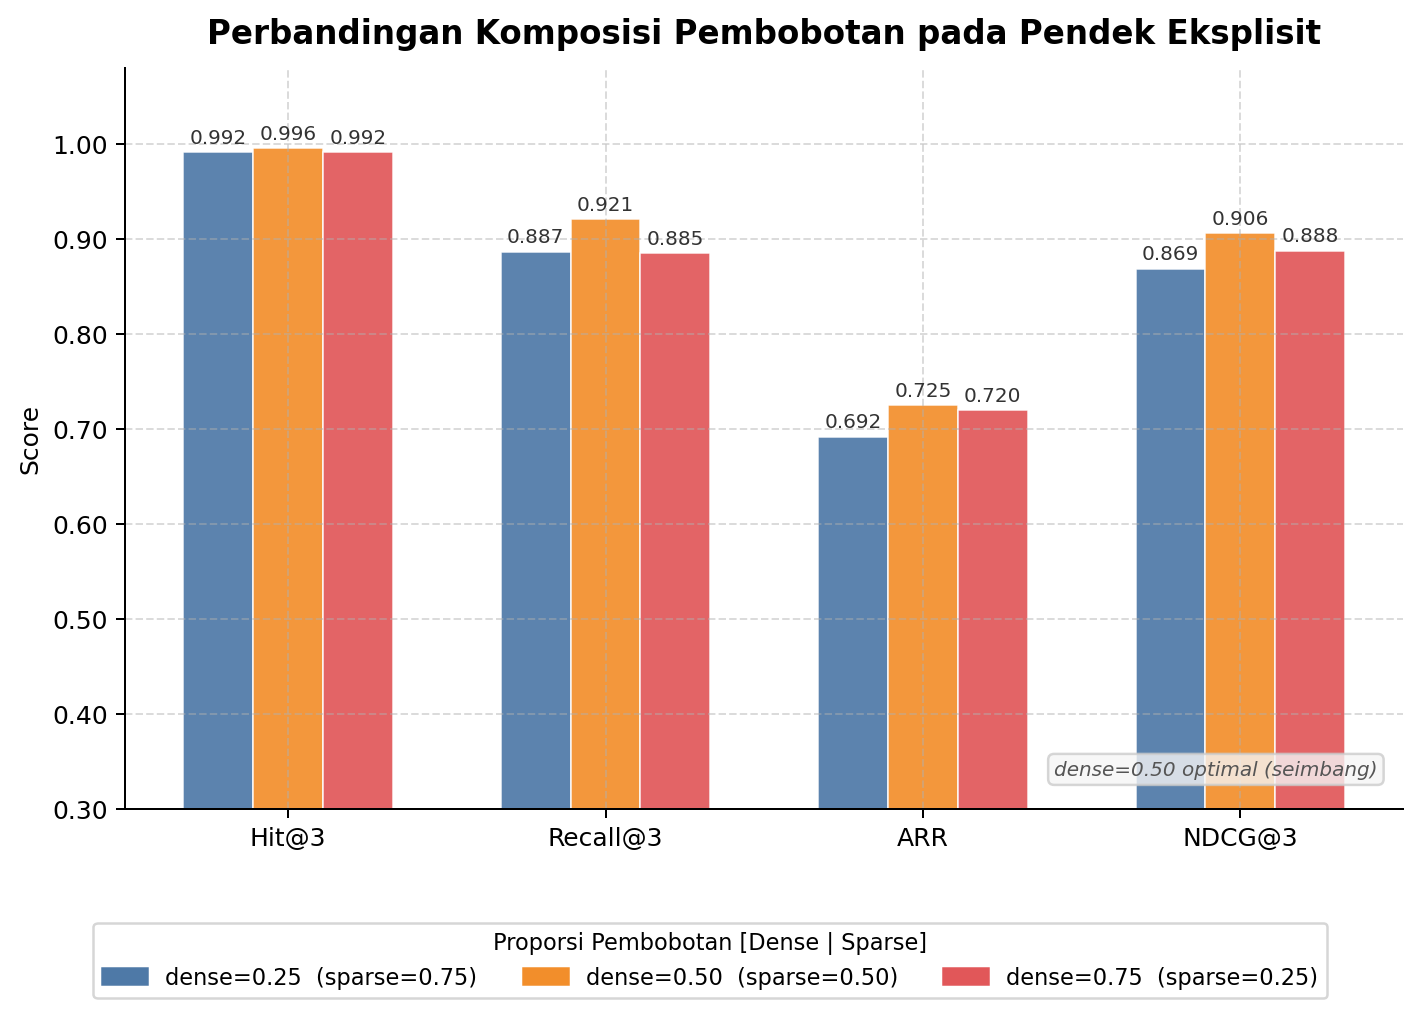
\includegraphics[width=0.85\textwidth]{Gambar/4.2.1.1/viz_A_eksplisit_short.png}
	\caption{Perbandingan metrik evaluasi berdasarkan komposisi \textit{dense-sparse} pada \textit{query} pendek eksplisit}
	\label{fig:komposisi_eksplisit_short}
\end{figure}

\textbf{Hasil pada \textit{Query} Panjang Eksplisit}

Komposisi dominan \textit{sparse} memberikan hasil lebih unggul pada metrik \textit{coverage}, dengan Hit@3 lebih tinggi 0.044 dan Recall@3 lebih tinggi 0.050 dibanding dominan \textit{dense}. Pada metrik \textit{rank-sensitive}, perbedaannya lebih kecil, tetapi dominan \textit{sparse} tetap sedikit lebih baik pada NDCG@3 sebesar 0.019, sedangkan ARR relatif setara. Hal ini menunjukkan bahwa \textit{query} eksplisit panjang lebih terbantu oleh pencocokan leksikal/\textit{sparse}.

\begin{figure}[H]
	\centering
	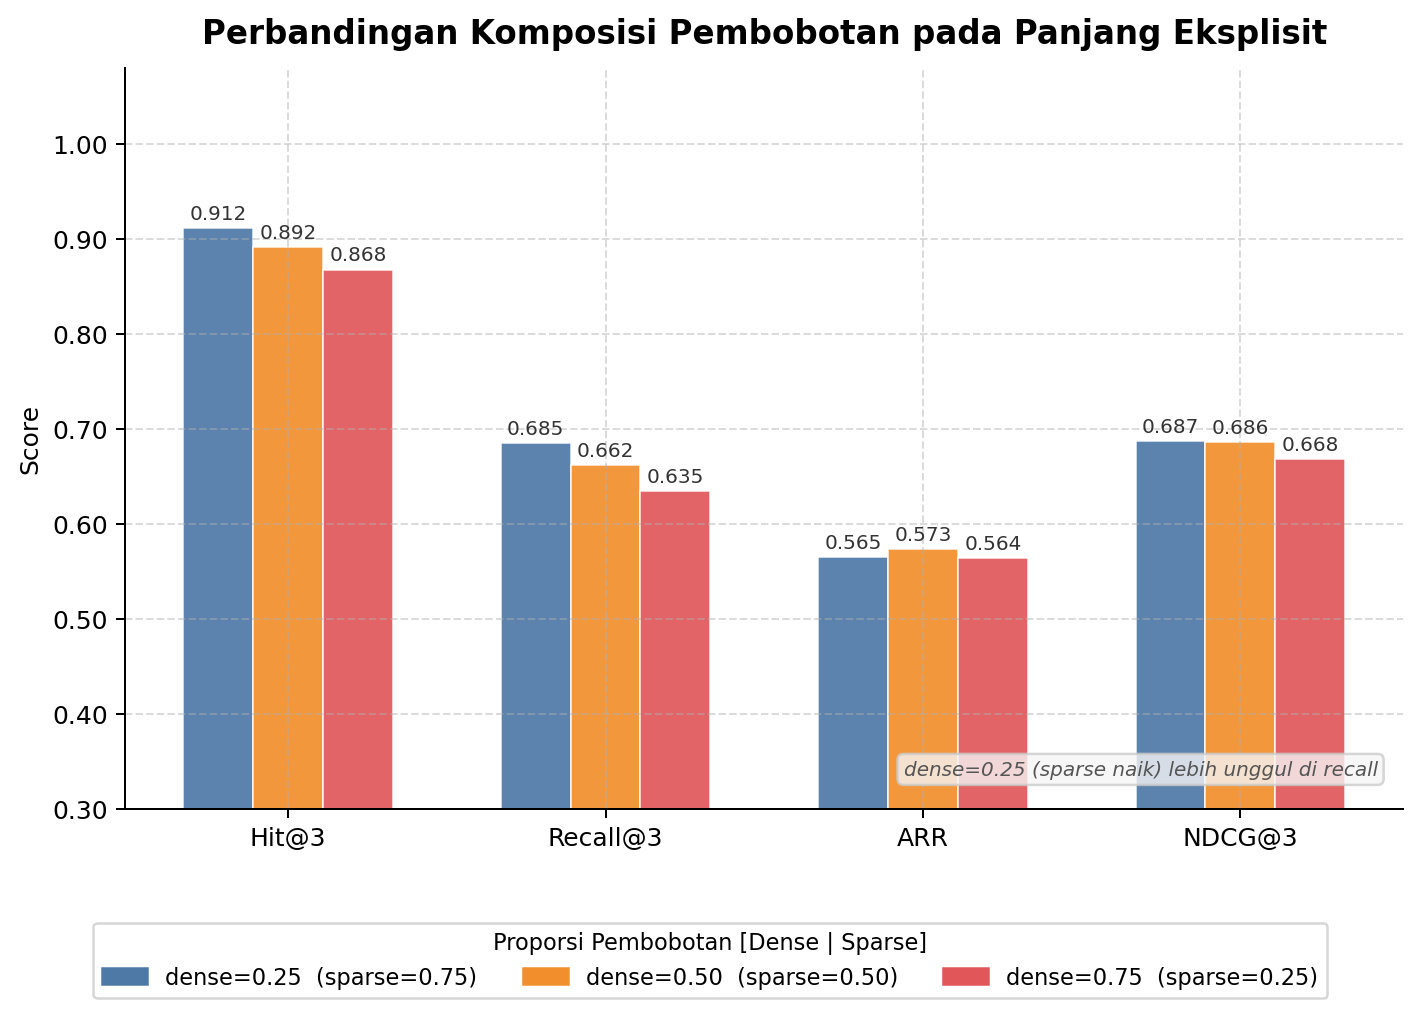
\includegraphics[width=0.85\textwidth]{Gambar/4.2.1.1/viz_A_eksplisit_long.png}
	\caption{Perbandingan metrik evaluasi berdasarkan komposisi \textit{dense-sparse} pada \textit{query} panjang eksplisit}
	\label{fig:komposisi_eksplisit_long}
\end{figure}

\textbf{Hasil pada \textit{Query} Pendek Implisit}

Komposisi seimbang 0.5:0.5 menjadi pembobotan terbaik pada seluruh metrik. Jika dibandingkan antara dominan \textit{sparse} dan dominan \textit{dense}, dominan \textit{sparse} sedikit lebih unggul, terutama pada ARR sebesar 0.015 dan NDCG@3 sebesar 0.013. Namun, peningkatan terbesar tetap diperoleh ketika \textit{dense} dan \textit{sparse} dikombinasikan secara seimbang.

\begin{figure}[H]
	\centering
	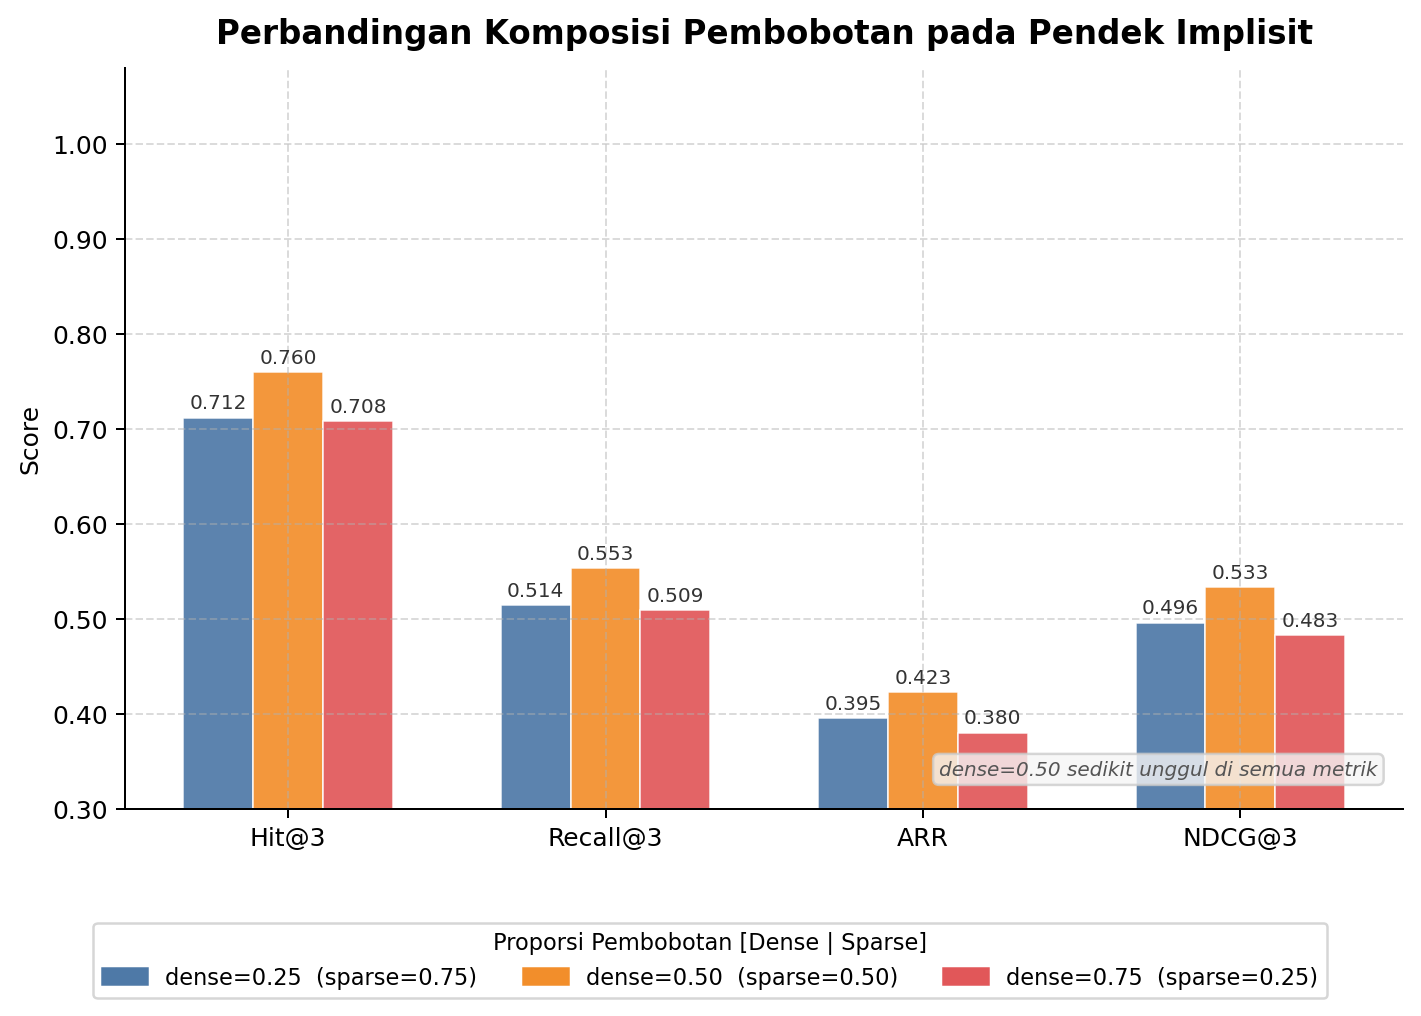
\includegraphics[width=0.85\textwidth]{Gambar/4.2.1.1/viz_A_implisit_short.png}
	\caption{Perbandingan metrik evaluasi berdasarkan komposisi \textit{dense-sparse} pada \textit{query} pendek implisit}
	\label{fig:komposisi_implisit_short}
\end{figure}

\textbf{Hasil pada \textit{Query} Panjang Implisit}

Komposisi seimbang 0.5:0.5 kembali menghasilkan performa terbaik pada seluruh metrik. Dominan \textit{sparse} juga lebih baik dibanding dominan \textit{dense}, dengan selisih Hit@3 sebesar 0.056, Recall@3 sebesar 0.052, ARR sebesar 0.045, dan NDCG@3 sebesar 0.058. Hasil ini menunjukkan bahwa dominasi \textit{dense} kurang optimal untuk \textit{query} implisit panjang, sementara kombinasi seimbang mampu menjaga cakupan sekaligus kualitas peringkat.

\begin{figure}[H]
	\centering
	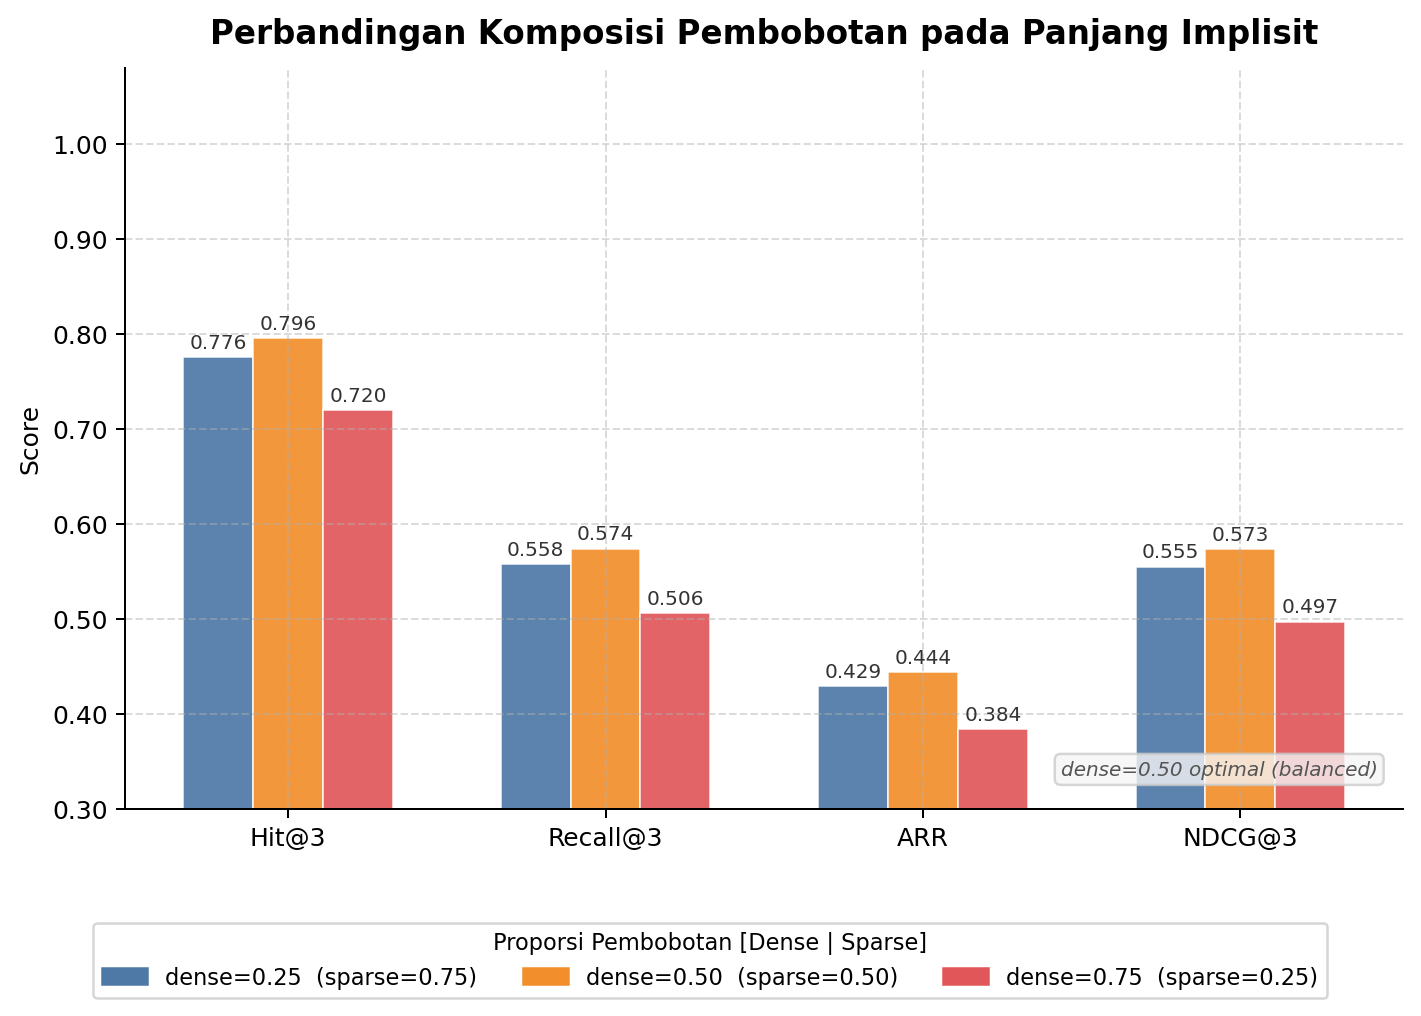
\includegraphics[width=0.85\textwidth]{Gambar/4.2.1.1/viz_A_implisit_long.png}
	\caption{Perbandingan metrik evaluasi berdasarkan komposisi \textit{dense-sparse} pada \textit{query} panjang implisit}
	\label{fig:komposisi_implisit_long}
\end{figure}

\subsubsection{Analisis Komparatif Jumlah \textit{Candidate Pool} pada \textit{Reranking Retrieval}}

\textbf{Hasil pada \textit{Query} Pendek Eksplisit}

\textit{Candidate pool} dengan ukuran terkecil, yaitu 5, konsisten memberikan nilai terbaik pada seluruh metrik dibanding \textit{pool} yang lebih besar. Metrik \textit{coverage} menunjukkan perbedaan kecil (Hit@3 = 0.004, Recall@3 = 0.014), sedangkan pada metrik \textit{rank-sensitive}, \textit{pool} 5 lebih unggul signifikan dengan ARR lebih tinggi 0.011 dan NDCG@3 lebih tinggi 0.013 dibanding \textit{pool} 10 hingga 20. \textit{Pool} 10, 15, dan 20 menghasilkan nilai yang hampir identik, sehingga penambahan kandidat di atas 10 tidak memberikan perbaikan.

\textbf{Hasil pada \textit{Query} Panjang Eksplisit}

\textit{Pool} 15 menjadi konfigurasi terbaik dengan unggul pada Hit@3 (0.968) dan ARR (0.582). Pola yang menarik adalah peningkatan kandidat dari \textit{pool} 5 ke 15 meningkatkan performa secara bertahap, namun \textit{pool} 20 justru menurun pada semua metrik. Penurunan ini menunjukkan bahwa terlalu banyak kandidat justru menurunkan kualitas \textit{reranking} pada \textit{query} eksplisit panjang, di mana \textit{noise} dari kandidat tambahan melemahkan akurasi peringkat.

\textbf{Hasil pada \textit{Query} Pendek Implisit}

\textit{Pool} 5 kembali memberikan performa terbaik pada seluruh metrik, dengan keunggulan yang lebih konsisten. Hit@3 lebih tinggi 0.032, Recall@3 lebih tinggi 0.048, ARR lebih tinggi 0.020, dan NDCG@3 lebih tinggi 0.031 dibanding \textit{pool} 20. Terlihat tren penurunan yang jelas seiring penambahan ukuran \textit{pool}, rata-rata penurunan konsisten terjadi pada setiap kenaikan \textit{step pool} (+5), yaitu Hit@3 turun rata-rata 0.019, Recall@3 turun 0.024, ARR turun 0.012, dan NDCG@3 turun 0.017 per \textit{step}. Hasil ini mengindikasikan bahwa \textit{query} implisit pendek sangat sensitif terhadap \textit{noise} dari kandidat tambahan.

\textbf{Hasil pada \textit{Query} Panjang Implisit}

\textit{Pool} 5 secara dominan mengungguli semua konfigurasi \textit{pool} lainnya pada seluruh metrik, dengan selisih yang paling besar dibanding tiga jenis \textit{query} sebelumnya. Hit@3 lebih tinggi 0.100, Recall@3 lebih tinggi 0.126, ARR lebih tinggi 0.094, dan NDCG@3 lebih tinggi 0.122 dibanding \textit{pool} 20. Rata-rata penurunan konsisten terjadi pada setiap kenaikan \textit{step pool} (+5), yaitu Hit@3 turun rata-rata 0.033, Recall@3 turun 0.042, ARR turun 0.031, dan NDCG@3 turun 0.041 per \textit{step}. Tren penurunan monoton yang tajam dari \textit{pool} 5 hingga \textit{pool} 20 menunjukkan bahwa \textit{query} implisit panjang sangat rentan terhadap degradasi akibat penambahan kandidat yang kurang relevan.

\begin{figure}[H]
	\centering
	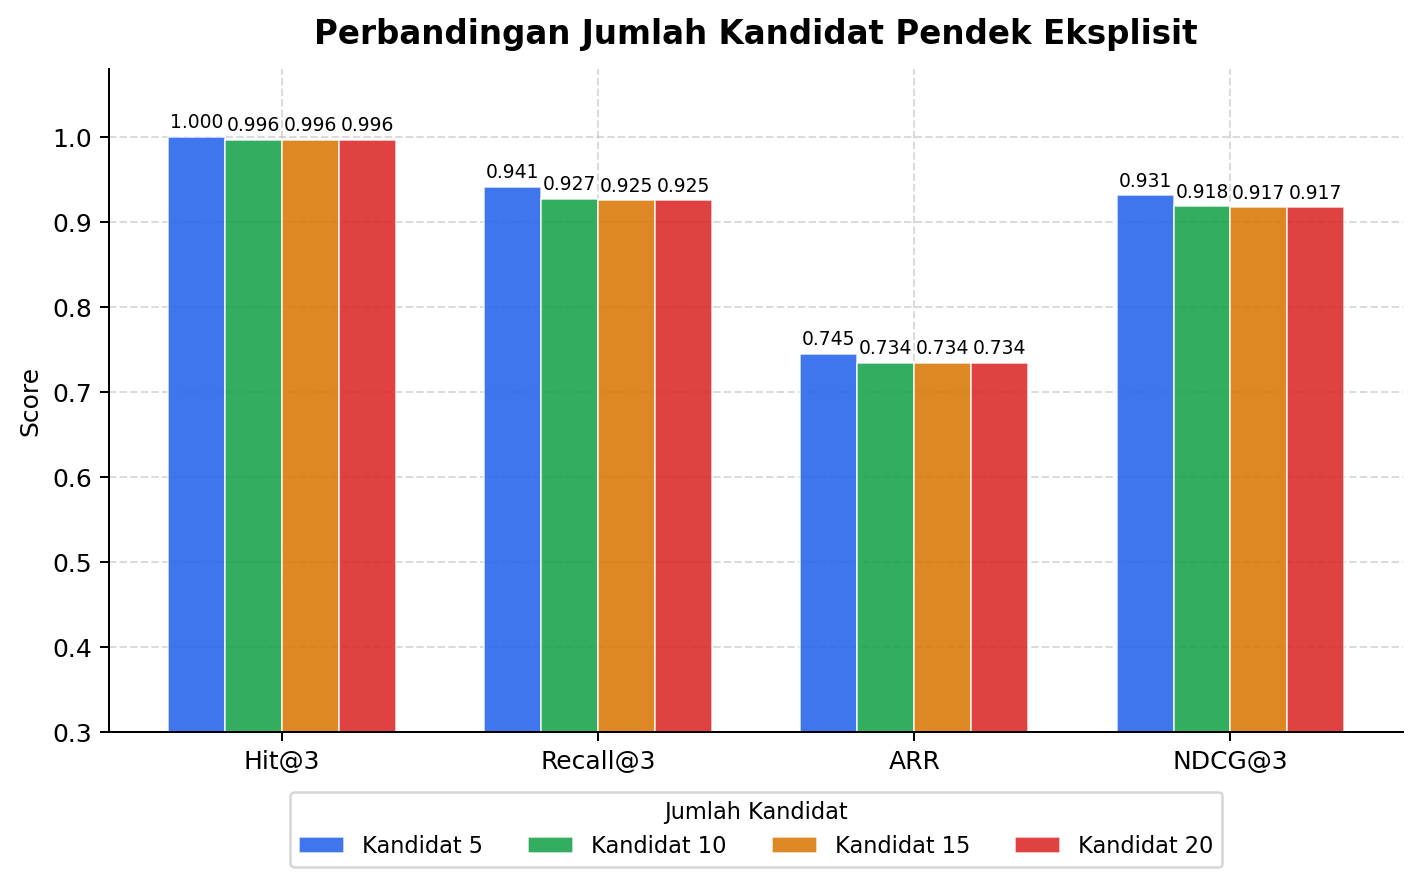
\includegraphics[width=0.85\textwidth]{Gambar/4.2.1.2/viz_optionA_eksplisit_short.png}
	\caption{Perbandingan metrik evaluasi berdasarkan ukuran \textit{candidate pool} pada \textit{query} pendek eksplisit}
	\label{fig:pool_eksplisit_short}
\end{figure}

\begin{figure}[H]
	\centering
	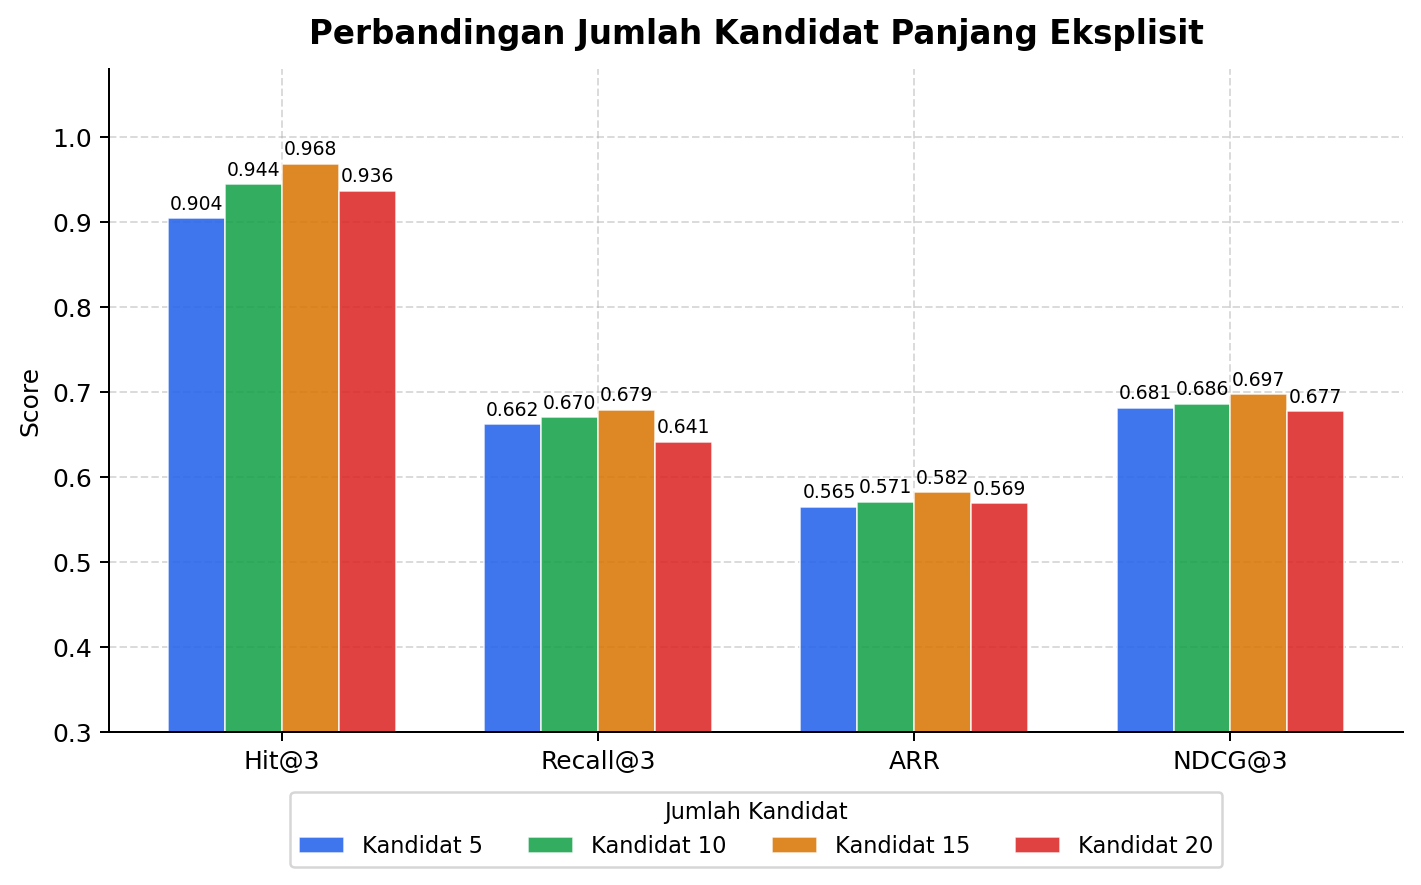
\includegraphics[width=0.85\textwidth]{Gambar/4.2.1.2/viz_optionA_eksplisit_long.png}
	\caption{Perbandingan metrik evaluasi berdasarkan ukuran \textit{candidate pool} pada \textit{query} panjang eksplisit}
	\label{fig:pool_eksplisit_long}
\end{figure}

\begin{figure}[H]
	\centering
	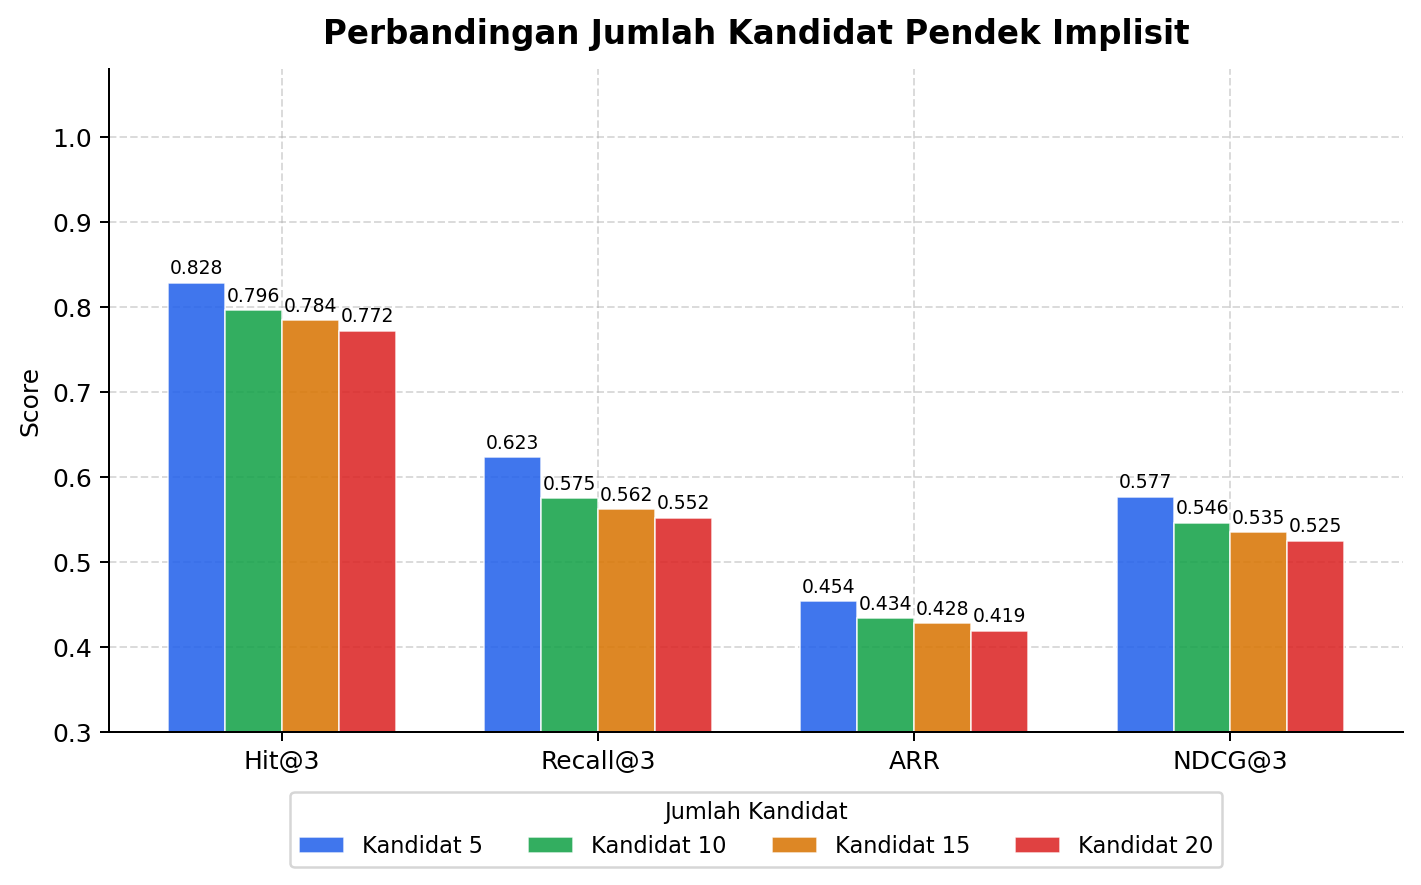
\includegraphics[width=0.85\textwidth]{Gambar/4.2.1.2/viz_optionA_implisit_short.png}
	\caption{Perbandingan metrik evaluasi berdasarkan ukuran \textit{candidate pool} pada \textit{query} pendek implisit}
	\label{fig:pool_implisit_short}
\end{figure}

\begin{figure}[H]
	\centering
	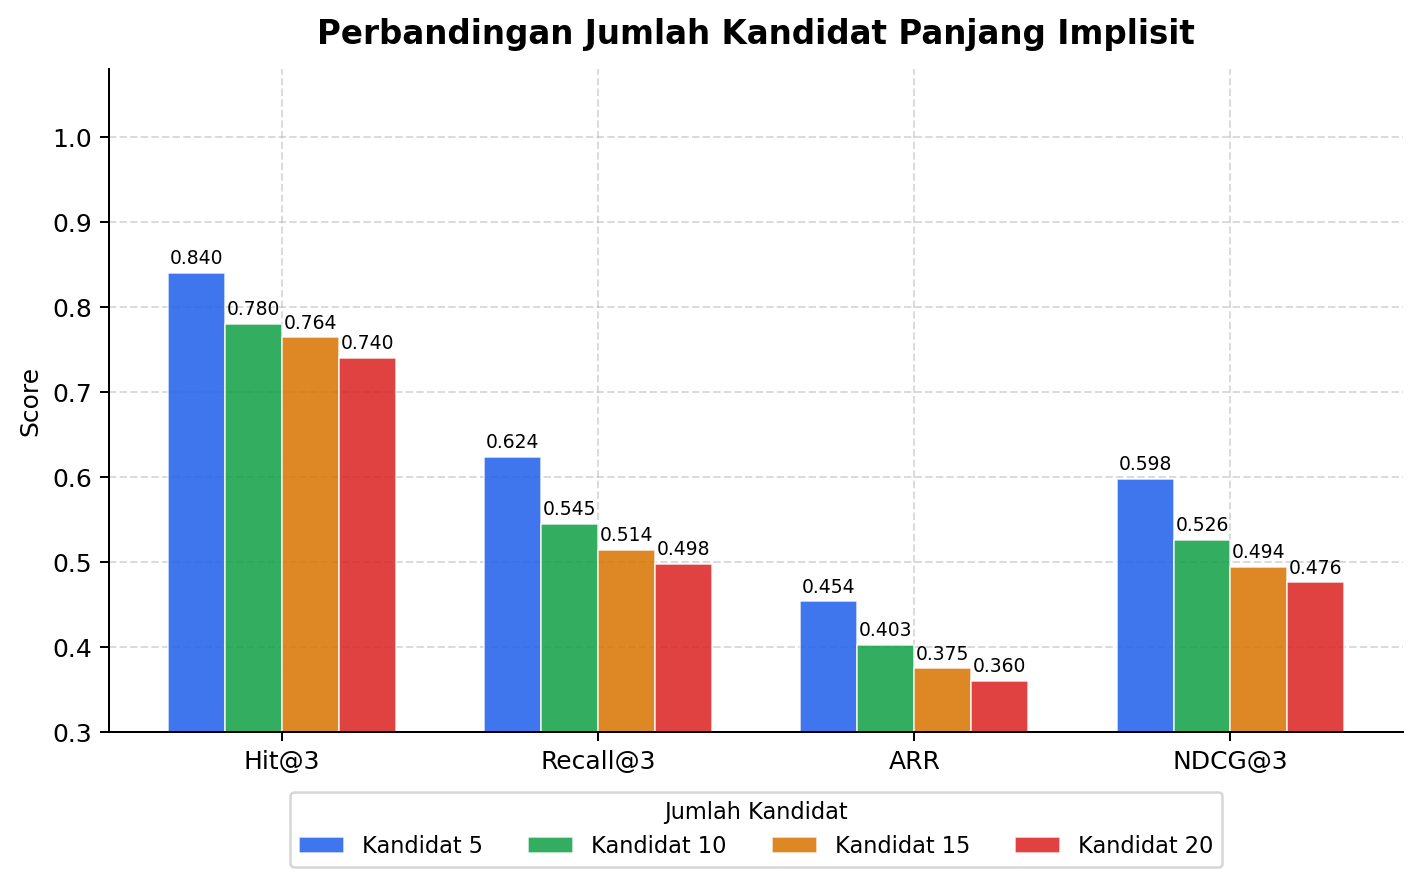
\includegraphics[width=0.85\textwidth]{Gambar/4.2.1.2/viz_optionA_implisit_long.png}
	\caption{Perbandingan metrik evaluasi berdasarkan ukuran \textit{candidate pool} pada \textit{query} panjang implisit}
	\label{fig:pool_implisit_long}
\end{figure}

\textbf{Hasil Waktu Latensi}

Berdasarkan rata-rata seluruh jenis \textit{query}, \textit{pool} 5 membutuhkan waktu 8.04 detik, \textit{pool} 10 meningkat menjadi 17.52 detik, \textit{pool} 15 menjadi 27.41 detik, dan \textit{pool} 20 mencapai 35.17 detik. Setiap penambahan 5 kandidat meningkatkan waktu rata-rata sekitar 9.49 detik dari \textit{pool} 5 ke 10, 9.89 detik dari \textit{pool} 10 ke 15, dan 7.75 detik dari \textit{pool} 15 ke 20. Hal ini menunjukkan bahwa semakin besar \textit{candidate pool}, semakin tinggi beban waktu proses \textit{reranking}.

\begin{figure}[H]
	\centering
	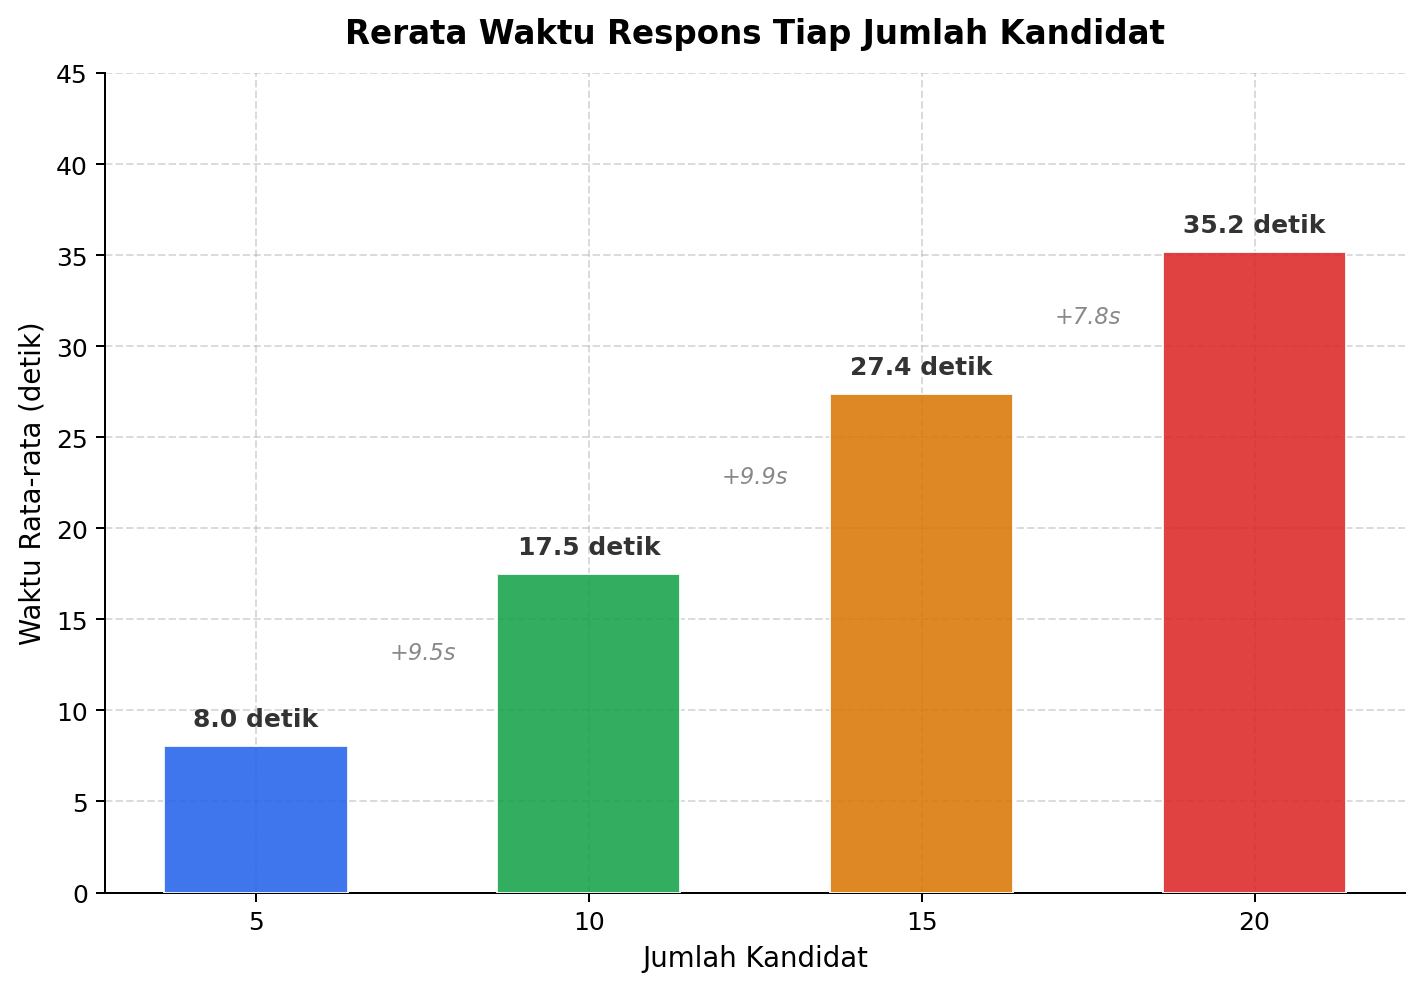
\includegraphics[width=0.85\textwidth]{Gambar/4.2.1.2/viz_time_per_pool.png}
	\caption{Perbandingan waktu latensi rata-rata berdasarkan ukuran \textit{candidate pool}}
	\label{fig:latensi_pool}
\end{figure}

\subsubsection{Analisis Komparatif Independen antara \textit{Hybrid Retrieval} dan \textit{Reranking}}

Perbandingan ini mengacu pada konfigurasi CE=0 (\textit{hybrid retrieval} dengan komposisi optimal 0.5:0.5) dan CE=1 (\textit{reranking retrieval} dengan \textit{pool} optimal 5). Secara umum, \textit{reranker} lebih unggul dibandingkan \textit{hybrid retrieval} pada sebagian besar jenis \textit{query}.

\textbf{Hasil pada \textit{Query} Pendek Eksplisit}

Metode \textit{Reranking} optimal dengan \textit{pool} 5 konsisten menghasilkan nilai terbaik pada seluruh metrik dibanding \textit{Hybrid Scoring} optimal komposisi 0.5:0.5. Keunggulan paling terlihat pada Recall@3 dan metrik \textit{rank-sensitive}, dengan Recall@3 lebih tinggi 0.020, ARR lebih tinggi 0.020, dan NDCG@3 lebih tinggi 0.025. Pada Hit@3, selisihnya relatif kecil yaitu 0.004, karena kedua metode sama-sama sudah mencapai cakupan yang sangat tinggi.

\textbf{Hasil pada \textit{Query} Panjang Eksplisit}

Performa \textit{Hybrid} dan \textit{Reranker} relatif seimbang pada \textit{query} eksplisit panjang. \textit{Reranker} sedikit lebih unggul pada Hit@3 sebesar 0.012, sedangkan Recall@3 menghasilkan nilai yang sama. Namun, pada metrik \textit{rank-sensitive}, \textit{Hybrid} sedikit lebih baik dengan ARR lebih tinggi 0.008 dan NDCG@3 lebih tinggi 0.005. Hal ini menunjukkan bahwa untuk \textit{query} eksplisit panjang, \textit{Hybrid} masih kompetitif dalam menjaga kualitas urutan dokumen.

\textbf{Hasil pada \textit{Query} Pendek Implisit}

\textit{Reranker pool} 5 memberikan peningkatan paling konsisten dibanding \textit{Hybrid} pada seluruh metrik. Selisih terbesar muncul pada metrik \textit{coverage}, yaitu Hit@3 lebih tinggi 0.068 dan Recall@3 lebih tinggi 0.070. Pada metrik \textit{rank-sensitive}, \textit{Reranker} juga unggul dengan ARR lebih tinggi 0.031 dan NDCG@3 lebih tinggi 0.044. Hasil ini menunjukkan bahwa \textit{reranking} membantu memperbaiki relevansi pada \textit{query} implisit pendek.

\textbf{Hasil pada \textit{Query} Panjang Implisit}

\textit{Reranker} kembali unggul pada seluruh metrik untuk \textit{query} implisit panjang. Dibanding \textit{Hybrid}, \textit{Reranker} meningkatkan Hit@3 sebesar 0.044 dan Recall@3 sebesar 0.050, sedangkan pada metrik \textit{rank-sensitive} ARR meningkat 0.010 dan NDCG@3 meningkat 0.025. Dengan demikian, \textit{Reranker} lebih efektif untuk \textit{query} implisit karena mampu menyaring kandidat yang lebih relevan setelah proses \textit{retrieval} awal.

\subsubsection{Analisis Komparatif Komposisi \textit{Scoring Hybrid Retrieval} dan \textit{Reranking}}

\textbf{Hasil pada \textit{Query} Pendek Eksplisit}

Komposisi dominan CE memberikan hasil lebih unggul pada metrik \textit{coverage}, dengan Recall@3 lebih tinggi 0.011 dibanding dominan \textit{Hybrid}, sedangkan Hit@3 relatif setara karena seluruh konfigurasi mencapai nilai 1.000. Pada metrik \textit{rank-sensitive}, dominan CE juga konsisten lebih baik, dengan ARR lebih tinggi 0.021 dan NDCG@3 lebih tinggi 0.021. Hal ini menunjukkan bahwa \textit{query} eksplisit pendek lebih terbantu oleh dominasi \textit{Cross-Encoder} dalam proses \textit{score fusion}.

\textbf{Hasil pada \textit{Query} Panjang Eksplisit}

Komposisi dominan \textit{Hybrid} memberikan hasil lebih unggul pada metrik \textit{coverage}, dengan Hit@3 lebih tinggi 0.004 dan Recall@3 lebih tinggi 0.015 dibanding dominan CE. Pada metrik \textit{rank-sensitive}, perbedaannya relatif kecil, di mana dominan CE sedikit lebih baik pada ARR sebesar 0.002, sedangkan dominan \textit{Hybrid} lebih unggul pada NDCG@3 sebesar 0.004. Namun, komposisi seimbang CE=0.50 menghasilkan ARR dan NDCG@3 terbaik, sehingga \textit{query} eksplisit panjang lebih optimal ketika bobot CE dan \textit{Hybrid} tidak terlalu dominan pada salah satu sisi.

\textbf{Hasil pada \textit{Query} Pendek Implisit}

Pada \textit{query} pendek implisit, konfigurasi dengan CE dominan (0.75) menghasilkan performa yang lebih baik pada metrik \textit{coverage}, sedangkan konfigurasi \textit{Hybrid} dominan lebih unggul pada metrik \textit{rank-sensitive}. Komposisi seimbang 0.5:0.5 kembali menjadi titik \textit{trade-off} yang optimal di antara keduanya.

\textbf{Hasil pada \textit{Query} Panjang Implisit}

Selain Hit@3 yang hasilnya relatif setara, komposisi seimbang 0.5:0.5 konsisten menghasilkan nilai terbaik pada metrik lainnya. Dominan \textit{Hybrid} sedikit lebih unggul pada Recall@3, sedangkan dominan CE sedikit lebih baik pada ARR dan NDCG@3. Hal ini mengonfirmasi bahwa keseimbangan bobot antara \textit{Hybrid} dan CE menghasilkan performa yang paling stabil pada \textit{query} implisit panjang.

\subsection{Analisis Hasil Eksperimen \textit{Query} Dokumen DTI}

\subsubsection{Analisis Komparatif Komposisi \textit{Dense} dan \textit{Sparse} pada \textit{Hybrid Retrieval}}

Sama seperti pada \textit{query} sintetis, proporsi 0.5:0.5 menjadi konfigurasi paling optimal untuk seluruh metrik kecuali Hit@3. Dominan \textit{sparse} selalu konsisten lebih baik dibanding dominan \textit{dense}, yang menunjukkan bahwa pencocokan leksikal tetap memiliki kontribusi penting pada dokumen DTI.

\subsubsection{Analisis Komparatif Jumlah \textit{Candidate Pool} pada \textit{Reranking Retrieval}}

Sama seperti pada \textit{query} sintetis, semakin banyak \textit{candidate pool} maka hasil akurasi menurun secara konsisten untuk keempat metrik evaluasi. \textit{Pool} 5 tetap menjadi konfigurasi terbaik yang meminimalkan \textit{noise} dan latensi tambahan.

\subsubsection{Analisis Komparatif Independen antara \textit{Hybrid Retrieval} dan \textit{Reranking}}

Berbeda dari \textit{query} sintetis yang lebih menguntungkan \textit{reranker}, pada kasus dokumen DTI komponen \textit{hybrid} lebih dominan dan menunjukkan performa yang lebih baik. Hal ini mengindikasikan bahwa karakteristik \textit{query} dari dokumen nyata DTI lebih sesuai dengan pendekatan \textit{hybrid retrieval} dibandingkan \textit{reranking} murni.

\subsubsection{Analisis Komparatif Komposisi \textit{Scoring Hybrid Retrieval} dan \textit{Reranking}}

Sejalan dengan hasil analisis independen, pada kasus dokumen DTI komponen \textit{hybrid} lebih dominan dalam proses \textit{score fusion}. Hal ini berbeda dengan pola pada \textit{query} sintetis yang lebih diuntungkan dengan dominasi \textit{Cross-Encoder}.
